\documentclass[11pt,a4paper]{article}
\usepackage{amsfonts,amssymb,tabularx, graphicx, hyperref}
\usepackage[left=3cm,right=3cm,top=2cm,bottom=2cm]{geometry}
\usepackage[parfill]{parskip}
\usepackage[utf8]{inputenc}
\usepackage{menukeys}
\usepackage{booktabs}% http://ctan.org/pkg/booktabs
\newcommand{\tabitem}{~~\llap{\textbullet}~~}

\author{Nguyen Chi Thanh, Manuel Schildknecht}
\title{EA GUI: Graphical User Interface for OpenEA}
\begin{document}
\maketitle

\section{Introduction}
\subsection{Context}
EA GUI is a part of the internship project of Bui Quang Minh, Nguyen Chi Thanh, Pham Nguyen Quang, Vo Huynh Quang Kiet and Manuel Schildknecht at the Frankfurt University of Applied Science, Germany. The project is about building a generic system for network optimization using evolutionary algorithm (EA). EA GUI provides an expandable graphical user interface as an add-on to the OpenEA Core Library to run customized EA using configuration file as input. This report describes the web version of the EA GUI.

\subsection{Requirements}
Basic information and requirements:

\begin{itemize}
\item Language: HTML5/CSS3/JavaScript (1.8.5)
\item Platform: Ubuntu 64 bit (16.4), Firefox (54.0)
\item Dependencies:

\begin{tabular}{ l l }
\tabitem $\texttt{npm} (3.5.2)$ 				& 	\tabitem $\texttt{bower} (1.8.0)$\\
\tabitem $\texttt{body-parser} (1.17.1)$		&	\tabitem $\texttt{angular-route} (1.6.4)$ \\
\tabitem $\texttt{cookie-parser} (1.4.3)$ 	& 	\tabitem $\texttt{material-design-icons} (3.0.1)$ \\
\tabitem $\texttt{debug} (2.6.3)$ 			& 	\tabitem $\texttt{angular-material} (1.1.4)$\\
\tabitem $\texttt{express} (4.15.2)$ 		& 	\tabitem $\texttt{angular-sanitize} (1.6.4)$\\
\tabitem $\texttt{fs-extra} (3.0.1)$ 		& 	\tabitem $\texttt{angular-scroll-glue} (2.2.0)$ \\
\tabitem $\texttt{meminfo} (0.0.0)$ 			& 	\tabitem $\texttt{angular-messages} (1.6.4)$	\\
\tabitem $\texttt{morgan} (1.8.1)$ 			& 	\tabitem $\texttt{angular-material-data-table} (0.10.10)$ \\
\tabitem $\texttt{randomstring} (1.1.5)$ 	& 	\tabitem $\texttt{underscore} (1.8.3)$ \\ 
\tabitem $\texttt{serve-favicon} (2.4.2)$	& 	\tabitem $\texttt{JQuery} (3.2.1)$		\\
\tabitem $\texttt{vis} (4.20.0)$				&	\tabitem $\texttt{amCharts3} (3.21.2)$ \\
\tabitem $\texttt{NodeJS} (6.11.0)$ 			&	\tabitem $\texttt{AngularJS} (1.6.4)$\\

\end{tabular}
\item Recommended IDE: Webstorm 2017.1.4
\end{itemize}

\subsection{Structure}

The EA-GUI folder will look like following if it was cloned from the repository:

\renewmenumacro{\directory}{pathswithfolder} 
\directory{EA-GUI}
\begin{itemize}

\item \texttt{app.js}: \texttt{JS} imports required modules, reads request and returns response
\item \texttt{install.sh}: installation script
\item \texttt{package.json}: \texttt{JSON} defines npm dependencies and start path
\end{itemize}

\directory{EA-GUI, bin, www}: the start up script of \texttt{npm}

\renewmenumacro{\directory}{pathswithfolder} 
\directory{EA-GUI, etc}

\directory{EA-GUI, node\_modules}: where npm libraries will be installed into

\directory{EA-GUI, proc}: stores information about running and previous process

\directory{EA-GUI, public}: stores all necessary components for the client-side of the web-app
\begin{itemize}
\renewmenumacro{\directory}{paths} 
\item \texttt{bower.json}: defines bower dependencies
\item \texttt{index.html}: index page of the web-app
\end{itemize}
\directory{EA-GUI, public, app}: consists of \texttt{HTML} and \texttt{JS} files for the web-app

\directory{EA-GUI, public, bower\_components}: where bower libraries will be installed into

\directory{EA-GUI, public, css}: stores the \texttt{css} file for the web-app

\directory{EA-GUI, public, etc}

\directory{EA-GUI, public, extra\_js}: stores extra \texttt{JS} files that are not installable via bower

\renewmenumacro{\directory}{pathswithfolder} 
\directory{EA-GUI, routes}
\begin{itemize}
\renewmenumacro{\directory}{paths} 
\item \texttt{exec.js}
\item \texttt{index.js}
\item \texttt{proc.js}
\end{itemize}

\section{Installation}
\subsection{Automatic Installation}

If the whole project was cloned from the online repository, the installation script should be located in \texttt{(project\_root\_folder)/EA-GUI/install.sh}. It must be executed in order to install all dependencies. The user can run the script by the following command lines:

\texttt{\$ cd (project\_root\_folder)/EA-GUI/}

\texttt{\$ chmod +x install.sh}

\texttt{\$ ./install.sh}

\subsection{Manual Installation}

The user can manually run the following command lines:

\texttt{\$ sudo apt install python-software-properties}

\texttt{\$ curl -sL https://deb.nodesource.com/setup\_6.x | sudo -E bash -}

\texttt{\$ sudo apt install nodejs}

\texttt{\$ sudo npm install -g bower}

\texttt{\$ sudo runuser -l "\$SUDO\_USER" -c "npm --prefix\symbol{92}"\$execpath/EA-GUI\symbol{92}" install}

\texttt{\symbol{92}"\$execpath/EA-GUI\symbol{92}""}

\texttt{\$ sudo runuser -l "\$SUDO\_USER" -c "npm --prefix \symbol{92}"\$execpath/EA-GUI/public\symbol{92}"}

\texttt{\$ install \symbol{92}"\$execpath/EA-GUI/public\symbol{92}""}

\texttt{\$ cd ./public}

\texttt{\$ bower install}

\section{Usages}

This section is written mainly for the user of the graphical user interface, which is shown in Figure 1. The appearance of the graphical user interface may vary depending on your screen resolution. The recommended screen resolution is 1280x720 or higher.

The GUI can be started using the following command:

\texttt{\$ openea gui}

Located on the left side of the web-app is the navigation bar, where the user can navigate him- or herself to the launch page, the graph viewer page or the currently running processes.

\subsection{Homepage or Launch page}
\begin{figure}[htp]
\centering
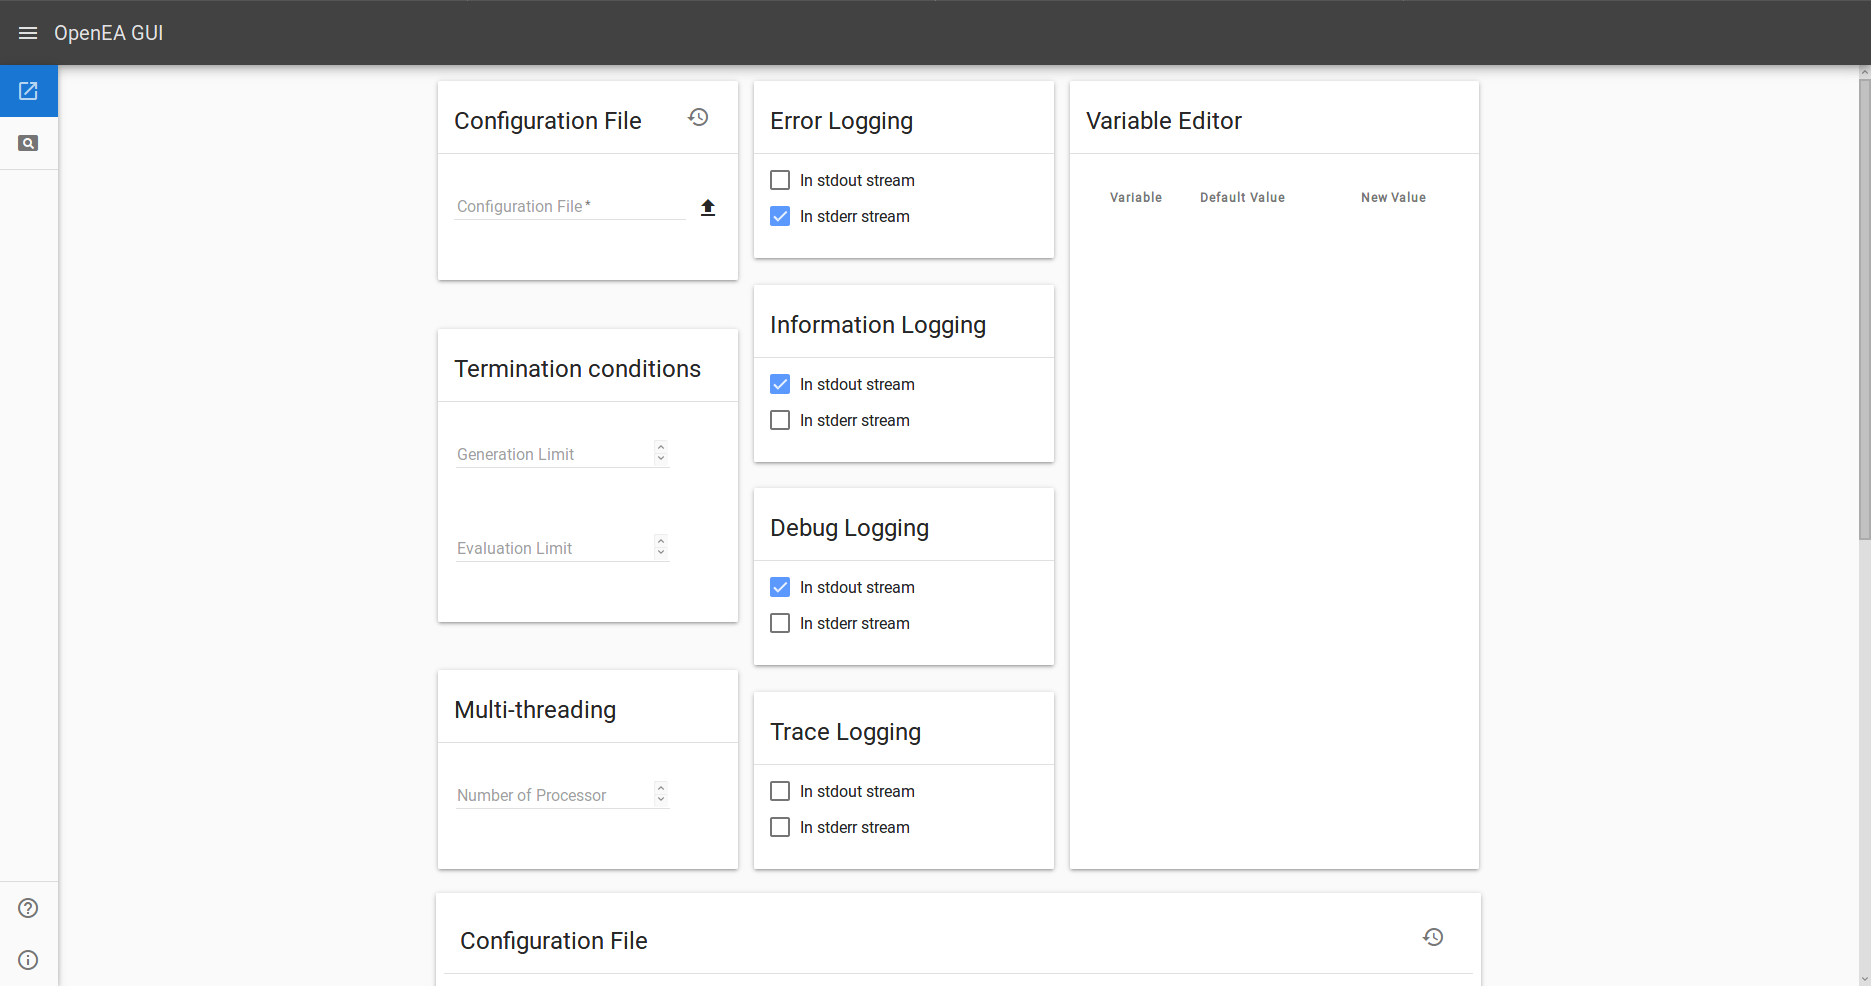
\includegraphics[scale=0.2]{/home/thanh/workspace/vgu_interns/EA-GUI/doc/pictures/prog.png}
\caption{Graphical User Interface}
\label{}
\end{figure}
The homepage (or launch page) is an configuration panel where the user can define the configuration file and relevant options and launch a new EA. The options are categorized so that the relevant options are located in the same \textbf{card}. Every card has two parts, the upper part is the \textit{card title}, where the name of the card and relevant function buttons (if available) are located, and the other part is where the options in that category located.

At the bottom of the page is the launch button to launch a new EA with the chosen configuration. By default, this button is disabled until all fields are valid. 

\subsubsection{File Chooser card}
This card acts as a file uploader that helps the user to choose the desired configuration file. In order to choose a file from the local machine, the user can simply click in the area of the \textit{Configuration File*} field, then the internal file chooser will pop up and ask the user to choose the desired file. To clear the field, the user can press the reset button on the top-right corner of the card. 
\begin{figure}[htp]
\centering
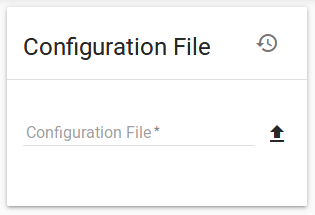
\includegraphics[scale=0.4]{/home/thanh/workspace/vgu_interns/EA-GUI/doc/pictures/filechooser.png}
\caption{File Chooser card}
\label{}
\end{figure}

\subsubsection{Termination Condition card}
This card consists of the fields for defining the limitation for generation or evaluation. The user can only input a positive integer into these two fields, otherwise the fields will be marked red indicating that the input is invalid and the user cannot start the EA with such input. 
\begin{figure}[htp]
\centering
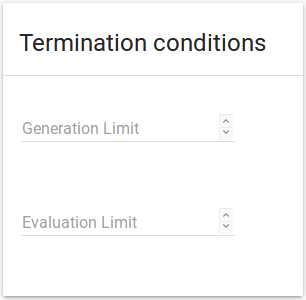
\includegraphics[scale=0.4]{/home/thanh/workspace/vgu_interns/EA-GUI/doc/pictures/termcondi.png}
\caption{Termination Condition card}
\label{}
\end{figure}

\subsubsection{Multi-threading card}
This field helps the user to define the number of threads for the EA. This field is blank by default.
\begin{figure}[htp]
\centering
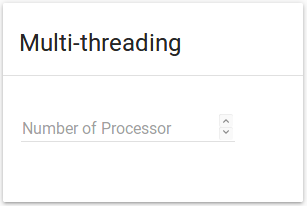
\includegraphics[scale=0.4]{/home/thanh/workspace/vgu_interns/EA-GUI/doc/pictures/thread.png}
\caption{Multi-threading card}
\label{}
\end{figure}

\subsubsection{Logging cards}
These cards provides the user with the options to show or hide specific logging levels, including \textit{error, information, debug} and \textit{trace}. There are two avaiable logging streams for the user to choose, namely \textit{standard output stream} (\texttt{stdout}) and \textit{standard error stream} (\texttt{stderr}). The user can choose to show one logging level in two streams at the same time by checking both boxes, and the user can also choose not to show one logging level by un-checking both boxes. By default, the \textit{Information} and \textit{Debug} levels are shown in \texttt{stdout}, the \textit{Error} level is shown in \texttt{stderr}, and the \textit{Trace} level is hidden.
\begin{figure}[htp]
\centering
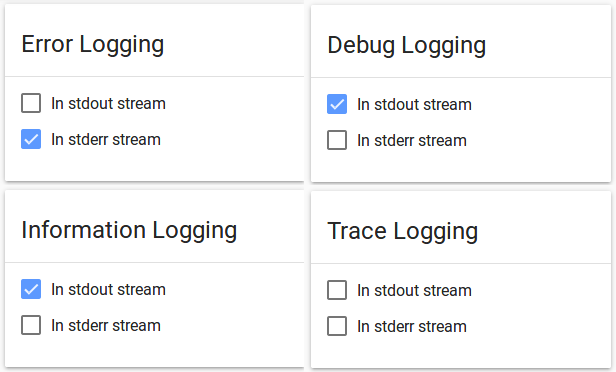
\includegraphics[scale=0.4]{/home/thanh/workspace/vgu_interns/EA-GUI/doc/pictures/logging.png}
\caption{Logging cards}
\label{}
\end{figure}

\subsubsection{Variable Editor card}
This card provides the user with the ability to edit the values of the available variables in the \texttt{eaml} file. The table will be filled after the user successfully chose a valid \texttt{eaml} file. There are three columns namely \textit{Variable}, \textit{Default Value} and \textit{New Value}. The first two columns are used as references to set the new values, therefore they are read-only by default. There is no feature to check if the input value is valid or not, therefore the user must be careful when using this table.
\begin{figure}[htp]
\centering
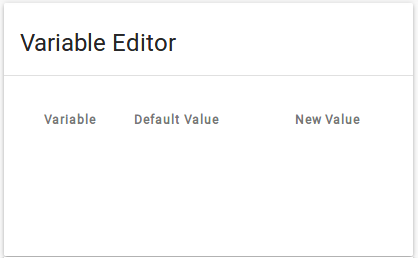
\includegraphics[scale=0.4]{/home/thanh/workspace/vgu_interns/EA-GUI/doc/pictures/vedit.png}
\caption{Variable Editor card}
\label{}
\end{figure}

\subsubsection{EAML Editor card}
This card provides the user with the ability to edit the whole \texttt{EAML} file without opening the local file viewer. The text field will be filled with the content of the \texttt{EAML} file once the user successfully chose a valid one. Changes in file content will only be avaiable in the scope of the web-app and do not (or cannot) affect the original file in the local machine. The user can get the edited \texttt{EAML} file belonging to a previous run EA by browsing the \texttt{proc} folder. 

The user can reset this field to the original content by pressing the top-right \textit{reset} button.
\begin{figure}[htp]
\centering
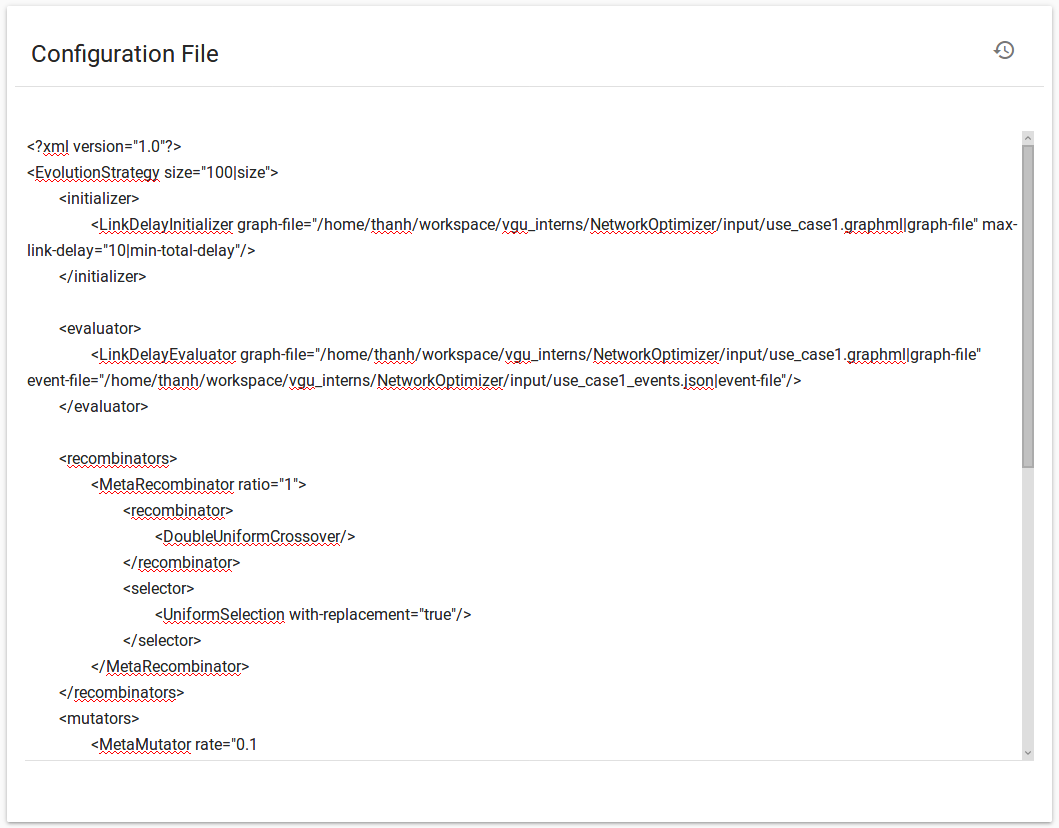
\includegraphics[scale=0.4]{/home/thanh/workspace/vgu_interns/EA-GUI/doc/pictures/eaml.png}
\caption{EAML Editor card}
\label{}
\end{figure}

\subsubsection*{EAML Modification Priority}
There are three ways that the user can modify a \texttt{EAML}. The first way is using a local script editor on the current machine, the second way is modifying the EAML editor field in the web-app and the last way is modifying the variable table. Out of these three ways, the variable editor has the most priority when it comes to modifying the EAML files, and the first way - modifying the \texttt{EAML} file itself - has the least priority. In the other words, the modifications in the variable editor will be considered first, then the eaml editor, then lastly the eaml file itself. Please bear in mind that after successfully choosing an eaml file and the eaml field is already ready, any local change in the eaml file does not affect this field, unless the user loads this file again.

\subsection{Graph Viewer page}
This page contains one card, called \textit{Graph Visualizer}. This card displays the graphML-files with help of nodes (dots) and edges (lines), to create a network graph.

In the top-left corner of the card is a button which will open the internal file chooser and ask the user
to choose the desired graphML-file. After the visualized graphML-file shows up at the middle of the card, a new button gets visible as well. This new button opens a drop-down list, which represents the node attributes of the graphML-file. With the help of these attributes and the button "cluster" at the top-right corner of the card, it is possible to cluster the network. For this purpose the cluster-button takes the selected attribute from the drop-down list and bind the nodes which correspond to this attribute to one node. One click at a clustered node will release all the bounded nodes to their original places at the card. The cluster-button will not work if there is no attribute selected.

It is possible to move the nodes in the visualization and hovering over a node or edge will display a tooltip in which every attribute of the hovered node or edge is shown.  

After a graphML-file is selected and shown at the screen a new file-chooser button will show up next to the first one. It asks the user to select a event.json-file. When a event-file is chosen the event will start and be shown with help of the visualized graph. Next to this file-chooser a button exist which toggles the Event so that it can be paused and started again.

At the very bottom of this card the events will be displayed as text. A scrollbar exists for the events so that the card stays at a normal size.    

\begin{figure}[htp]
\centering
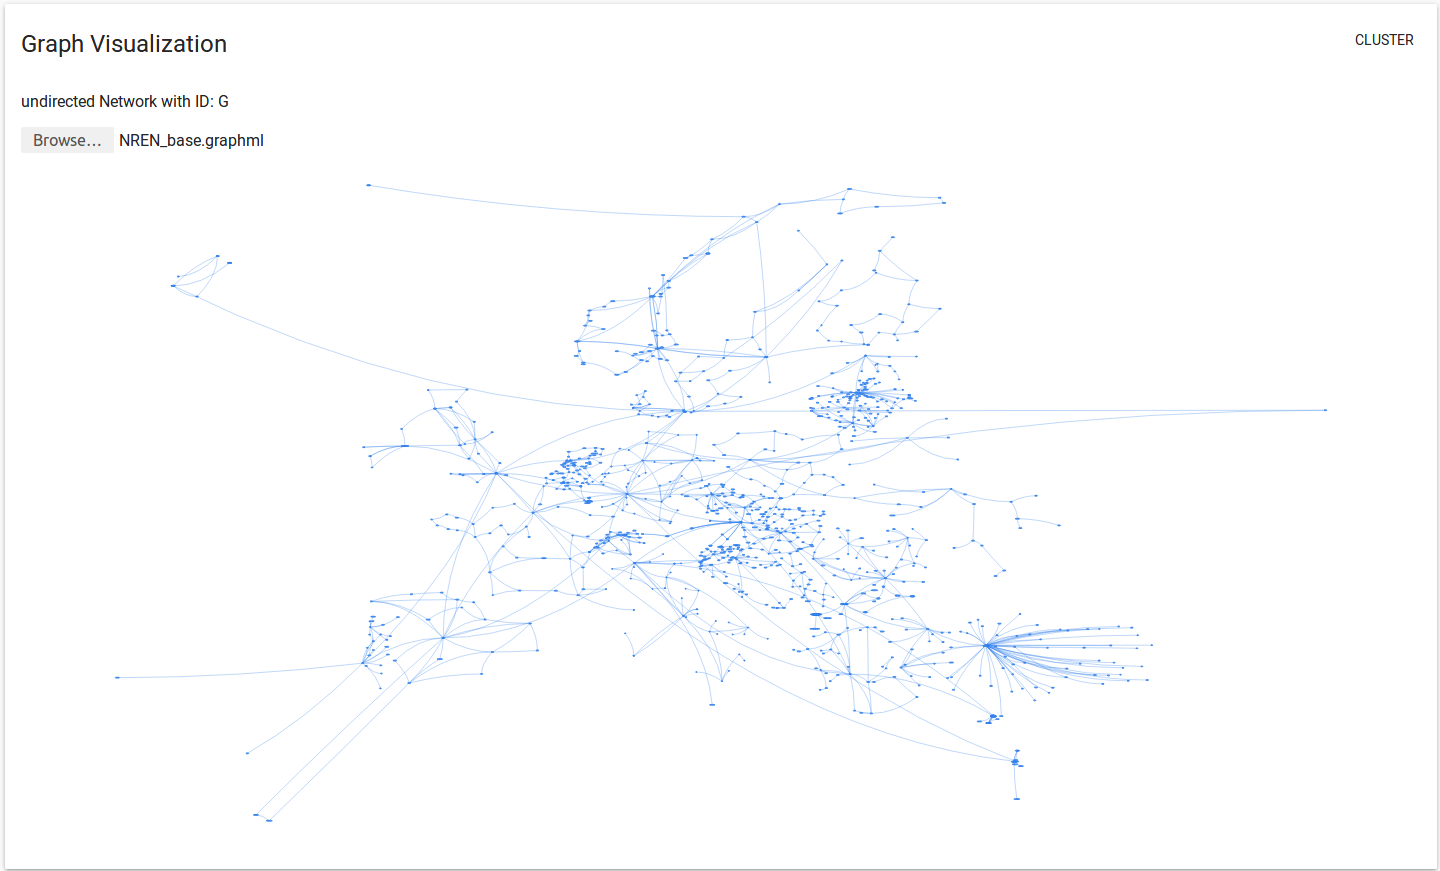
\includegraphics[scale=0.3]{/home/thanh/workspace/vgu_interns/EA-GUI/doc/pictures/graph.png}
\caption{Graph Viewer}
\label{}
\end{figure}

\subsection{Process page}
This page will be created once all configurations have been set and a new EA is started. The page consists of a console on the top, a fitness plot card on the bottom left and a graph visualization card on the right. If the EA is running, the console and the fitness plot is updated in real-time. If the EA has finished, the console will store the old information, and the fitness plot will stop updating itself. Once the EA has finished and the user tries to navigate between the sites, the fitness plot will not work when he or she get back to that same page again.

The graph visualization is exactly the same to the one seen in the graph viewer page, please see Section 3.2 for the description.
\subsubsection{Console card}
This card imitates the linux terminal and shows the information on the current EA. If the EA is running, the console is updated real-time. There are two buttons and two switches on the card header, including the show/hide button for hiding and showing the console, the stop button for stopping the EA and the switches for toggling show/hide the \texttt{stdout} and \texttt{stderr} streams.
\begin{figure}[htp]
\centering
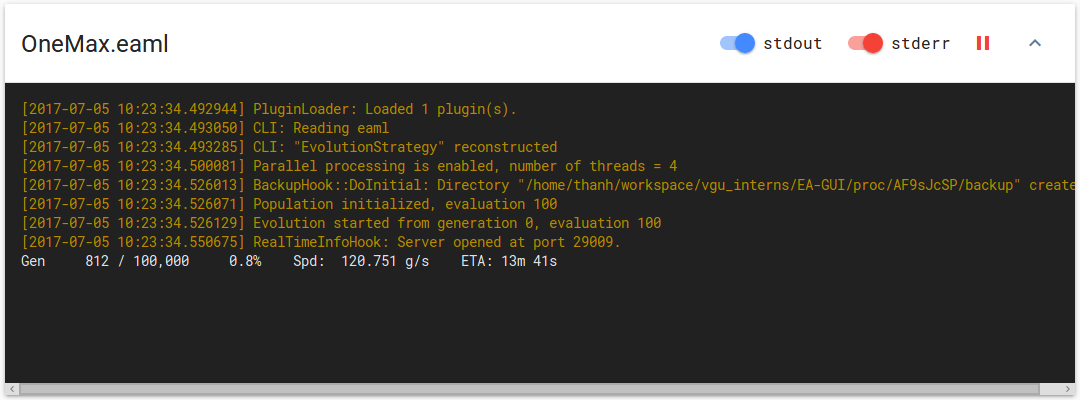
\includegraphics[scale=0.3]{/home/thanh/workspace/vgu_interns/EA-GUI/doc/pictures/console.png}
\caption{Console card}
\label{}
\end{figure}
\subsubsection{Fitness Plot card}
This card displays the fitness values of the EA in real-time to a statistical diagram. In the top-right corner of the card are three buttons. Two of them the "Select" and the "Pan" button are select-buttons. If "Select" is pressed a preciser area of the statistical diagram can be selected. To move freely in the diagram "Pan" should be chosen. The third button is an update-button, which will stop newer values to enter the diagram. A second click on this button will rescind the first one and the diagram will draw new values again. At the bottom-left corner of this card, the values of all lines in the statistic are displayed as the sum of all values that are currently displayed at the diagram. As a result the sum of the values will decrease if a preciser area is selected. If the mouse is hovered over an area at the diagram, a tooltip will be displayed which shows the values of this area. At last there exist a button at the top-right corner of the diagram, which will only be visible if not the whole statistic is selected. Then the button "show all" can be pressed and the complete statistic will be shown.
\begin{figure}[htp]
\centering
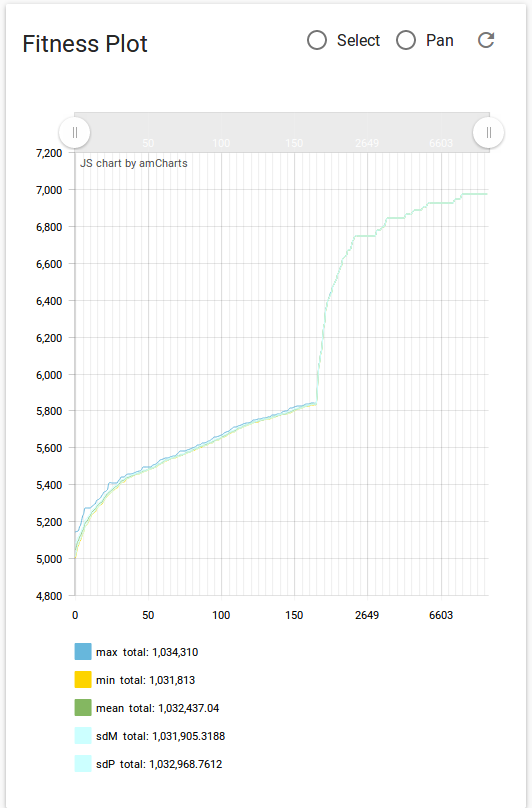
\includegraphics[scale=0.3]{/home/thanh/workspace/vgu_interns/EA-GUI/doc/pictures/fitness.png}
\caption{Fitness Plot card}
\label{}
\end{figure}
\end{document}
